%%%%%%%%%%%%%%%%%%%%%%%%%%%%%%%%%%%%%%%%%%%%%%%%%%%%%%%%%%%%%%%%%%%%%%%%%%%%%%%%%%%%%%
% Key Concept IV       
%%%%%%%%%%%%%%%%%%%%%%%%%%%%%%%%%%%%%%%%%%%%%%%%%%%%%%%%%%%%%%%%%%%%%%%%%%%%%%%%%%%%%%

\newpage

\section{Key Concept IV \tiny Zeitliche Darstellung bei Simulation}

\begin{minipage}{0.6\textwidth}
	\begin{tabular}{l}
		$\cdot$ Die Simulation / Funktionstest wird mit Hilfe einer Test-Banch gemacht \\
		$\cdot$ Die Test-Banch sollte Wiederverwendbarsein \\
		$\cdot$ Test-Bench unabhängig des verwendeten verfahren des DUT \\
		$\cdot$ Um so früher ein Fehler bemerkt wird desto "`billiger"' ist er  \\
		$\cdot$ VHDL-Simulatoren arbeiten mit einer Event-Queue (sie Bild) \\
		$\cdot$ (SPICE-Simulatoren arbeiten mit DGL {\tiny $\rightarrow$ brauchen viel mehr Rechenleistung}) \\
		$\cdot$ Delta-Zyklus: (auf Bild t's) \\
		\qquad 1. Update Request: \qquad wartet auf Trigger\\
		\qquad 2. Prozessausfürung: \quad führt alle Prozesse aus {\tiny bis zum nächsten "`wait"'}\\
		\qquad 3. Signalzuweisung: \qquad neue Signale werden zugewiesen\\
		$\cdot$ Transport-Delay: rechnet die delays der Logikgatter ein \\
		$\cdot$ Internal-Delay: simuliert die Trägheit der Elektronik \\
	\end{tabular}
	
	\begin{minipage}{0.04\textwidth}
		\text{ } %platzhalter
	\end{minipage}
	\begin{minipage}{0.9\textwidth}
		\begin{VHDL}
B <= transport A after tp; 		-- tp in type "time"
D <= inertial C after tp;  		-- "inertial " nicht noetig\end{VHDL}
	\end{minipage}
	
\end{minipage}
\begin{minipage}{0.4\textwidth}
	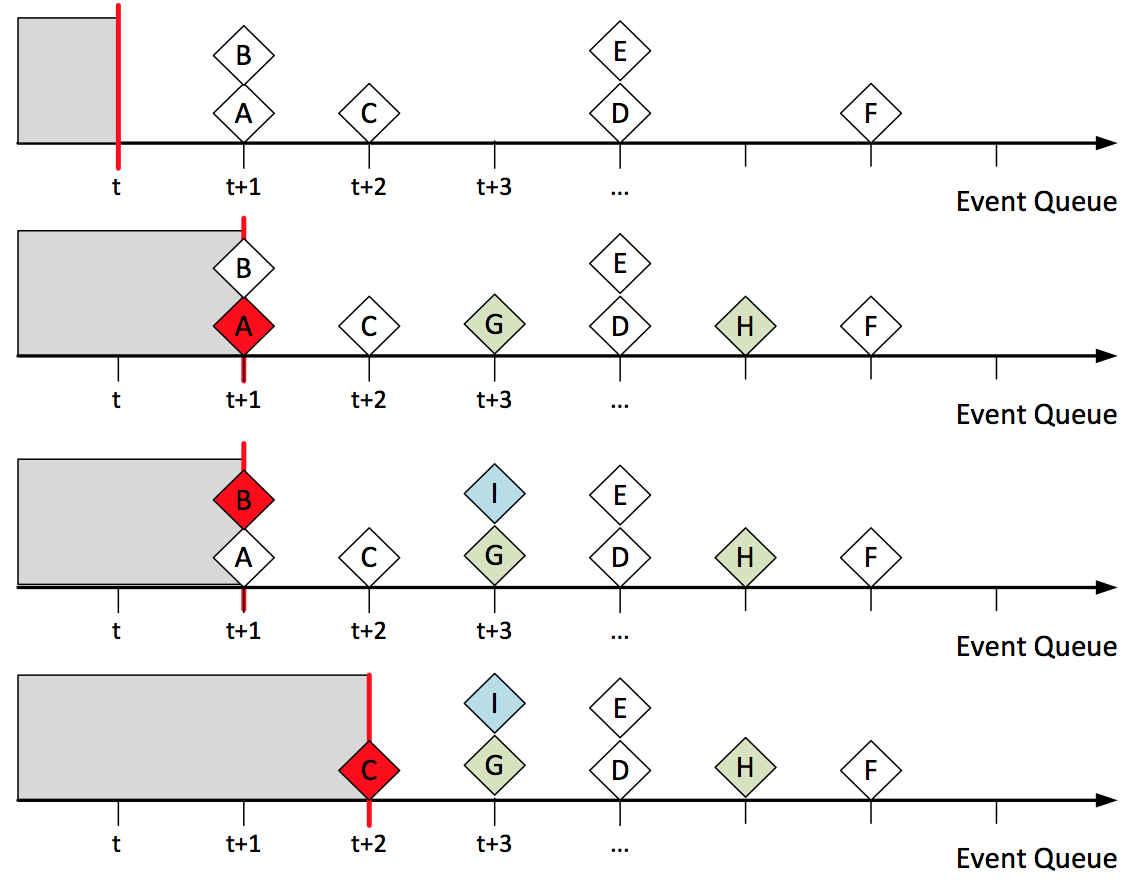
\includegraphics[width=\textwidth]{./bilder/EventQueue}
\end{minipage}

\begin{minipage}{0.4\textwidth}
	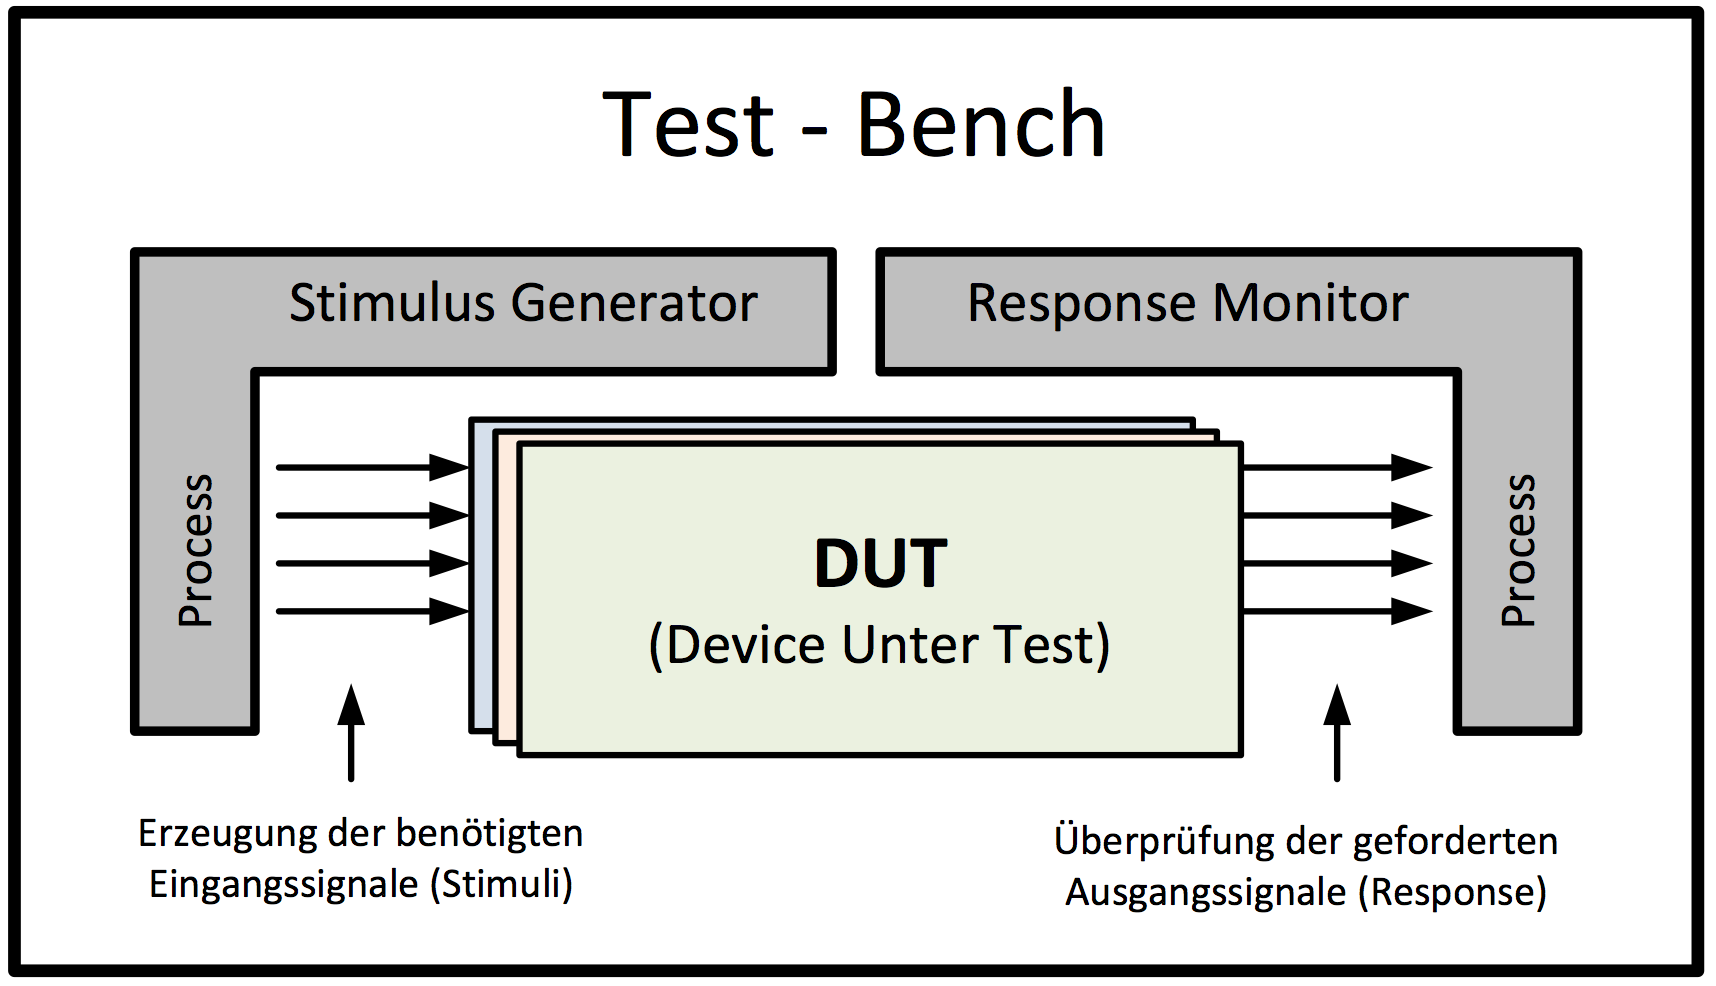
\includegraphics[width=\textwidth]{./bilder/TestBench}
\end{minipage}
\begin{minipage}{0.6\textwidth}
	\begin{tabular}{l}
		$\cdot$ In Test-Benchs werden oft Schleifen eingesetzt \\
		$\cdot$ Sie muss nicht Synthesefähig sein  \\
		$\cdot$ Automatische Überprüfung mit ASSERTs \\
		$\cdot$ Eine Test-Banch sollte eine leere entity haben {\tiny $\rightarrow$ keine Schnittstelle nach aussen}  \\
		$\cdot$ "`Simuli"' Eingang des DUT's, "`Respons"' erwartete Antwort\\
		$\cdot$ DUT "`1 zu 1"' aus work - library\\
	\end{tabular}
	
	\begin{minipage}{0.02\textwidth}
		\text{ } %platzhalter
	\end{minipage}
	\begin{minipage}{0.52\textwidth}
		\begin{VHDL}
-- for loop
[label:] for <parameter> in <range> loop
	{sequential statements}
end loop [label];
-- assert
[label:] assert condition [report string_expretion]
	[severity warning | error | ..];\end{VHDL}
	\end{minipage}
	\begin{minipage}{0.02\textwidth}
		\text{ } %platzhalter
	\end{minipage}
	\begin{minipage}{0.38\textwidth}
		\begin{VHDL}
-- Bsp fuer RST und CLK
rst <= '1', '0' after 150ms;
CLOCK : process
begin 
	clk <= '0';
	wait for (PERIOD / 2);
	clk <= '1';
	wait for (PERIOD / 2);
end process CLOCK;\end{VHDL}
	\end{minipage}
\end{minipage}


